\documentclass[preview]{standalone}

\usepackage{amsmath}
\usepackage{amssymb}
\usepackage{stellar}
\usepackage{bettelini}

\hypersetup{
    colorlinks=true,
    linkcolor=black,
    urlcolor=blue,
    pdftitle={Biologia},
    pdfpagemode=FullScreen,
}

\begin{document}

\title{Biologia}
\id{biologia-anatomia-fisiologia-cellula}
\genpage

\begin{snippetdefinition}{cellula-procariota-definizione}{Cellula procariota}
    Le \textit{cellule procariote} sono il tipo più semplice di cellule.
\end{snippetdefinition}

\begin{snippetdefinition}{cellula-eucariota-definizione}{Cellula eucariota}
    Le \textit{cellule eucariote} sono cellule
    che possiedono:
    \begin{itemize}
        \item \textit{organelli} o \textit{organuli}: sono strutture provviste di membrana;
        \item \textit{nucleo}: un organello contenente i cromosomi;
        \item sistemi di membrane interne.
    \end{itemize}
\end{snippetdefinition}

\begin{snippet}{24b7ecd4-99aa-417e-b0bd-50be9f5b8337}
    Le cellule procariote sono prive di un nucleo e di organelli.

    Le prime forme di vita erano unicamente cellule precariote.
    Essi svolgono esclusivamente la glicolisi e non la respirazione cellulare.
    Si muovono utilizzando dei \textit{flagelli} posto all'estremità della cellula.
\end{snippet}

\begin{snippet}{prok-euka-illustration}
    \begin{center}
    \begin{figure}[th]
        \centering
        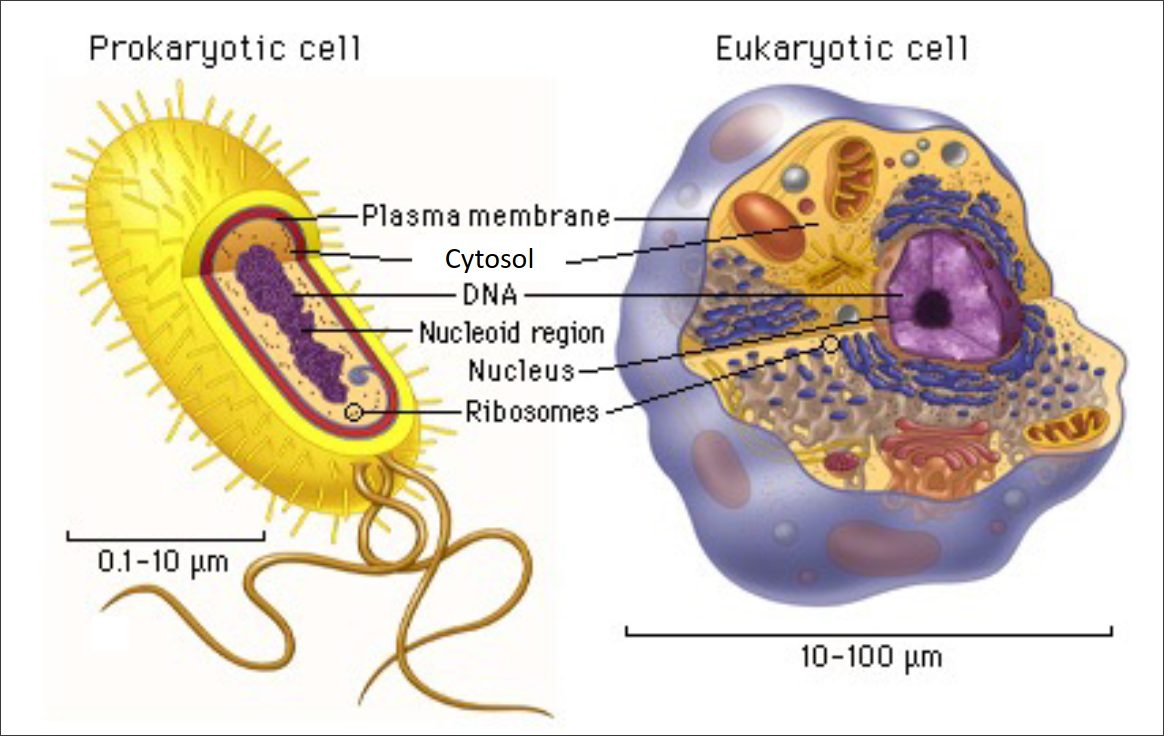
\includegraphics[width=0.75\textwidth]{./resources/prok-euka.png}
    \end{figure}
    \end{center}
\end{snippet}

\begin{snippetdefinition}{citosol-definizione}{Citosol}
    Con \textit{citosol} si intende la sostanza solvente presente nella cellula.
\end{snippetdefinition}

\begin{snippetdefinition}{citplasma-definizione}{Citplasma}
    Con \textit{citoplasma} si intende l'intera soluzione presente nella cellula.
\end{snippetdefinition}

\begin{snippetdefinition}{spermatozoo-definizione}{Spermatozoo}
    Gli \textit{spermatozoi} sono delle cellule eucariote pieni di mitocondri.
\end{snippetdefinition}

\begin{snippet}{dimensione-cellula-expl}
    Se la cellula fosse troppo grande, avrebbe un rapporto area su volume troppo piccolo, e non riuscirebbe
    a fare sufficientemente scambi sulla sua area superficiale.
    Per esempio, l'ovulo ad esempio deve essere grande per dare
    abbastanza materia energetica al feto prima che si
    formi la placenta.
\end{snippet}

\end{document}